\section{Sequences}
\label{sec:successioni}

A \emph{sequence}%
\mymargin{sequence}%
\index{sequence} in a set $X$ is a function $\vec a\colon \NN \to X$.
The set of functions $\NN \to X$ is usually denoted by $X^\NN$, and thus we
could write $\vec a \in X^\NN$.
Indeed, a sequence $\vec a$ can be interpreted as an infinite sequence of
elements of $X$:
\mynote{%
We use bold to emphasize that $\vec a$ is not a number but a \emph{list} (or
vector) of numbers.
In handwritten notation, bold is not possible, but we could underline the
variable name by writing $\underline a$ instead of $\vec a$.
Alternatively, one could write $\stackrel{\rightarrow}a$ or avoid any
distinction and simply write $a$.}
\[
  \vec a = (a_0, a_1, a_2, \dots, a_n, \dots )
\]
where it is understood that
\[
   a_n = \vec a(n).
\]
The components $a_n$ are called the \emph{terms} of the sequence.
The numbers $n$ are called \emph{indices}.
The entire sequence $\vec a$ can be denoted by $(a_n)_{n=0}^\infty$ or
$(a_n)_n$, or more simply by $a_n$ when it is clear that the entire sequence
$\vec a$ is intended and not a single term of it.%

For us, the most interesting case will be that of \emph{real sequences} $a_n\in
\RR$, i.e., the case $X=\RR$. However, we will also consider the case of
\emph{complex sequences} $a_n\in \CC$ (thus $X=\CC$) because this may be useful
in certain situations.%
\mynote{In some texts, sequences are denoted by the notation $\ENCLOSE{a_n}$, which is misleading because a sequence in $X$ is not simply a subset of $X$: the order in which the elements are taken is relevant.}

\subsection{Limit of a Sequence}

Since $\vec a \colon \NN\to\RR$ (or in $\CC$) is a function with domain
$\NN\subset \RR$ and since $+\infty$ is the only accumulation point of $\NN$, it
will be possible to consider the limit
\[
  \ell = \lim_{n\to +\infty} \vec a(n)
\]
which we could also write using one of the following notations:
\[
\ell = \lim \vec a = \lim_n a_n = \lim_{n\to +\infty} a_n
\]
or more concisely:
\[
  a_n \to \ell. 
\]

By explicitly stating the abstract definition of a limit, we observe that if
$(\alpha,+\infty]$ is a neighborhood of $+\infty$ with $\alpha>0$, its
intersection with $\NN$ (the domain of the function) is the set $\ENCLOSE{n\in
\NN\colon n> N}$ where $N=\lfloor \alpha \rfloor$ is a natural number. Thus, if
$\ell \in \RR$, the condition $a_n \to \ell$ is explicitly stated as follows:
\begin{equation}\label{eq:limite_successione_convergente}
\forall \eps>0\colon \exists N\in \NN\colon n>N\implies \abs{a_n-\ell} < \eps.  
\end{equation}
The condition $a_n\to +\infty$ is written as
\[
  \forall \alpha\in \RR \colon \exists N\in \NN \colon n>N \implies a_n > \alpha  
\]
and finally $a_n\to-\infty$ becomes
\[
  \forall \alpha\in \RR \colon \exists N\in \NN \colon n>N \implies a_n < -\alpha.    
\]

\begin{definition}[character of a sequence]
Let $a_n$ be a sequence with real or complex values, and consider the limit 
\[
  \lim_n a_n.  
\]
If such a limit exists, we will say that the sequence $a_n$ is 
\emph{regular}%
\mymargin{regular}%
\index{regular},
\index{sequence!regular}%
if the limit exists and is finite, we will say that the sequence is 
\emph{convergent}%
\mymargin{convergent}%
\index{convergent}%
\index{sequence!convergent}
if the limit is infinite, we will say that the sequence is 
\emph{divergent}%
\mymargin{divergent}%
\index{divergent}%
\index{sequence!divergent}
if the limit does not exist, we will finally say that the sequence is
\emph{indeterminate}%
\mymargin{indeterminate}%
\index{indeterminate}%
\index{sequence!indeterminate}.

We thus have the following alternatives:
\begin{enumerate}
 \item the sequence is convergent (has a finite limit);
 \item the sequence is divergent (has an infinite limit);
 \item the sequence is indeterminate (has no limit).
\end{enumerate}
Determining the \emph{character}
\mymargin{character of a sequence}%
\index{character!of a sequence}%
\index{sequence!character}%
of a sequence means specifying to which of the three categories it belongs.
\end{definition}

\begin{exercise}
A complex sequence $z_n\in \CC$ can be written in the form $z_n = x_n + i y_n$
where $x_n$ and $y_n$ are real sequences. It can then be verified that $z_n\to
z$ for $z\in \CC$ if and only if $x_n\to x$ and $y_n\to y$ where $z=x+ iy$ with
$x,y\in \RR$.
\end{exercise}

Note that a sequence $a_n\in \RR \subset \CC$ can be interpreted both as a real
sequence and as a complex sequence. The conditions for convergence in $\RR$ or
$\CC$ are then equivalent. However, if $a_n \to \infty$ (in $\bar \CC$) means
that $\abs{a_n}\to +\infty$, it may happen that $a_n$ does not have a limit of
either $+\infty$ or $-\infty$ because it could frequently change sign (an
example is $a_n = (-n)^n$).

In general, we might have sequences defined only on a subset $\NN$ of natural
numbers. As long as the sequence is defined in a neighborhood of $+\infty$
(i.e., from a certain $n_0$ onwards), this has no consequence on the limit as
$n\to +\infty$ (thanks to the locality of the limit,
theorem~\ref{th:localita_limite}).

\begin{example}
  The sequence $a_n = 1/n$ is defined for $n\in \NN$ but $n\neq 0$.
    This does not prevent us from studying its limit like any other sequence. To
  highlight the fact that the first index is $n=1$, the notation
  $(a_n)_{n=1}^\infty$ can be used.
\end{example}
 
\subsection{Bounded Sequences}
\label{sec:successione_limitata}%

If we have a real sequence $a_n$, we can also consider the operators:
\[
  \sup_n a_n, \qquad 
  \inf_n a_n, \qquad 
  \max_n a_n, \qquad 
  \min_n a_n 
\]
which are defined as for any other function. 
We know that $\sup$ and $\inf$ always exist (in $\bar\RR$), while $\max$ and
$\min$ may not exist.

The concept of boundedness for a sequence is inherited from the same concept
valid for functions.
A sequence $a_n$ (with real or complex values) is said to be 
\emph{bounded}%
\mymargin{bounded}%
\index{bounded} if 
the set $\{\abs{a_n}\colon n \in \NN\}$ is bounded. That is, if 
\[
\sup_n \abs{a_n} < +\infty.  
\]
\mynote{note that even when $a_n$ is complex, the sequence of moduli $\abs{a_n}$ is real (and non-negative).
We will see later that sequences with complex values do not create many more
difficulties than those that take negative values.
The real advantage will be with sequences with positive values, which is why the
modulus of a sequence is often considered.
}
Otherwise, the sequence is said to be \emph{unbounded}%
\mymargin{unbounded}%
\index{unbounded}.
These definitions apply as they are to sequences of complex numbers (replacing
the absolute value with the modulus).

If the sequence has real values, we can also talk about 
\emph{upper boundedness} when $\sup a_n <+\infty$ 
and \emph{lower boundedness} when $\inf a_n > -\infty$.


\begin{example}
Consider $a_n = \frac{1}{n+1}$ defined for $n\in \NN$.
Then
\[
  \sup a_n = \max a_n = 1, \qquad
  \inf a_n = 0, \qquad \text{there is no }\min a_n.
\]
\end{example}
\begin{proof}
For every $n \in \NN$, we have $n+1\ge 1$, and therefore $a_n = 1/(n+1) \le 1$.
Since $a_0 = 1$, we immediately obtain that $\max a_n = 1$, and consequently
$\sup a_n = 1$.

To verify that $\inf a_n = 0$, we must first verify that $0$ is a lower bound,
and this is true because $a_n = 1/(n+1)> 0$ since $n+1\ge 1 \ge 0$.
Furthermore, we must verify that for every $\eps >0$, there exists $n\in \NN$
such that $a_n < 0 + \eps = \eps$. This happens if $1/(n+1) < \eps$, i.e., if $n
> 1/\eps -1$, for example, for $n=\lceil 1/\eps\rceil$.
We have thus verified that $\inf a_n = 0$.
The minimum of $a_n$ does not exist because if it did, it should be equal to the
infimum, i.e., it should be $0$. But this is impossible because for every $n\in
\NN$, we have $a_n = 1/(n+1)\neq 0$.
\end{proof}

Since the set $\NN$ on which sequences are defined has a unique accumulation
point $+\infty$, if the sequence is convergent, it cannot be unbounded, as
expressed in the following.

\begin{theorem}[boundedness of convergent sequences]
  \label{th:limitatezza_successione_convergente}%
\mymark{**}%
If a sequence (real or complex) is convergent, then it is also bounded.
If a real sequence diverges to $+\infty$, then it is lower bounded; if it
diverges to $-\infty$, it is upper bounded.
\end{theorem}
%
\begin{proof}
  By the definition of limit~\eqref{eq:limite_successione_convergente}, 
  if $a_n\to \ell$ with $\ell$ finite, we know 
  that by choosing $\eps=1$, there must exist $N\in \NN$ such that 
  \[
      \forall n>N\colon \abs{a_n - \ell} < 1.
  \]
  Now observe that the indices $n$ for which $n\le N$ are finite in number 
  (in fact, they are $N+1$), and therefore there exists
  \[
   M = \max_{n\le N} \abs{a_n} 
   = \max \ENCLOSE{\abs{a_0}, \abs{a_1}, \dots , \abs{a_N}}.  
  \]
  Thus, choosing $R=\max\ENCLOSE{\abs{\ell}+1,M}$, 
  if $n\le N$, we certainly have $\abs{a_n}\le M \le R$,
  and if $n>N$, we still have, by the triangle inequality,
  \[
  \abs{a_n} \le \abs{a_n-\ell} + \abs{\ell} < 1+ \abs{\ell} \le R.  
  \]
  Therefore, overall, it results that $\sup_n \abs{a_n}\le R$, and the sequence 
  is bounded.

  If $a_n\to +\infty$, by the definition of limit, 
  choosing $(0,+\infty]$ as a neighborhood of $+\infty$, 
  there must exist an index $N\in \NN$ such that if $n>N$, we have $a_n>0$. 
  But then, setting $R=\min\ENCLOSE{0, a_0,\dots,a_N}$,
  we will have $a_n\ge R$ for every $n\in \NN$, and thus the sequence 
  is lower bounded.

  A similar proof is done in the case $a_n\to -\infty$.
\end{proof}


% \begin{theorem}[product of bounded by infinitesimal]
% \mymark{**}%
% \mymargin{product of bounded by infinitesimal}%
\index{product of bounded by infinitesimal}%
% If $a_n$ is a bounded sequence and $b_n\to 0$, then
% $a_n\cdot b_n \to 0$ (the result holds for both real 
% and complex sequences).
% \end{theorem}
% %
% \begin{proof}
%   If $a_n$ is bounded, it means there exists $R>0$ such that $\abs{a_n}\le R$ for
%   every $n\in \NN$.
%   If $b_n\to 0$, we know that also $\abs{b_n}\to 0$, thus
%   \[  
%     0
%     \le \abs{a_n\cdot b_n} 
%     = \abs{a_n}\cdot \abs{b_n} 
%     \le R\cdot \abs{b_n}\to R\cdot 0 = 0.
%   \]
%   By the squeeze theorem, we deduce that $\abs{a_n\cdot b_n}\to 0$, 
%   and therefore $a_n\cdot b_n \to 0$.
% \end{proof}

\subsection{Monotonic Sequences}

Definitions~\ref{def:monotonia} apply to sequences. 
We have thus already defined what it means for a sequence to be 
increasing, decreasing, strictly increasing, strictly decreasing,
monotonic, constant. For example, a sequence $a_n$ is said to be 
increasing if $n\ge m$ implies $a_n \ge a_m$.

The verification of the monotonicity of a sequence can be demonstrated 
more easily than in the general case of functions because 
we can use the principle of induction, as shown in the following theorem.


\begin{theorem}[monotonic sequences]
  \mymark{***}%
A sequence $a_n$ is
\begin{enumerate}
\item \emph{increasing}: if for every $n\in \NN$, we have $a_{n+1} \ge a_n$;
\item \emph{decreasing}: if for every $n\in \NN$, we have $a_{n+1} \le a_n$;
\item \emph{strictly increasing}: if for every $n\in \NN$, we have $a_{n+1}>a_n$;
\item \emph{strictly decreasing}: if for every $n\in \NN$, we have
$a_{n+1}<a_n$;
\end{enumerate}
\end{theorem}
%
\begin{proof}
  Consider, for example, the first condition (increasing function).
Obviously, if $a_n$ is increasing, we have $a_{n+1}\ge a_n$ because $n+1 > n$.
Conversely, suppose that for every $n\in \NN$, we have $a_{n+1}\ge a_n$.  Then
clearly $a_1\ge a_0$, $a_2\ge a_1 \ge a_0$, $a_3 \ge a_2 \ge a_1 \ge a_0$...
By induction, it can be shown that  $a_n \ge a_{n-1} \ge \dots \ge a_2
\ge a_1$.

The other cases are handled similarly.
\end{proof}

\begin{example}
  The sequence $a_n = n!$ is increasing 
  because for every $n$, we have $(n+1)! = (n+1)\cdot n! \ge n!$.
\end{example}

The monotonicity of a sequence is of extreme importance because,
as stated in the following theorem, monotonic sequences are regular, 
i.e., they always have a limit (finite or infinite). 
This theorem will be used many times, especially when we want 
to prove that a sequence has a limit but do not know the explicit value 
of the limit. 
The first notable example is in Theorem~\ref{th:5767684}, where we define 
the constant $e$ as the limit of a particular increasing sequence.

\begin{theorem}[regularity of monotonic sequences]
\label{th:limite_successione_monotona}%
Monotonic sequences are regular.
More precisely, if $a_n$ is increasing, then $\lim a_n = \sup a_n$; 
if $a_n$ is decreasing, then $\lim a_n = \inf a_n$.
\end{theorem}
\begin{proof}
In reality, this theorem is a special case of 
Theorem~\ref{th:limite_funzione_monotona} if we remember that a sequence 
$a_n$ is nothing but a function $f(n)=a_n$ defined on natural numbers.
And the limit at $+\infty$ is a left limit.
Given the importance of this result, we can repeat the proof 
in this specific case.

To fix ideas, suppose the sequence $a_n$ is increasing and prove 
that $\lim a_n = \ell$ with $\ell=\sup a_n$.
By the definition of limit, we must verify that for any neighborhood $U$ 
of $\ell$, we have $a_n\in U$ definitively.
We will actually prove a stronger condition, namely that $a_n$ is definitively 
in a left neighborhood of $\ell$, i.e., for every $q<\ell$, there exists $N$
such that
for every $n\ge N$, we have $a_n\in (q,\ell]$ (note that $\ell$ can be finite or
$+\infty$,
and what we have written holds in both cases).
That $a_n\le \ell$ is obvious because $\ell=\sup a_n$ is, by definition, an
upper bound
of $a_n$. Moreover, $\ell$ is the minimum of the upper bounds, and therefore,
given
$q<\ell$, we know that $q$ is not an upper bound, i.e., there must exist $N$
such that
$a_N > q$. But, being $a_n$ increasing, we know that for every $n\ge N$, we have
$a_n \ge a_N >q$, and this concludes the proof.
\end{proof}

%%%%%%%%%%%%%%%%%
%%%%%%%%%%%%%%%%%
%%%%%%%%%%%%%%%%%
%%%%%%%%%%%%%%%%%

\subsection{Recursive Sequences}

Recursive sequences are sequences
defined by induction (via theorem~\ref{th:induzione}):
\[
 \begin{cases}
   a_0 = \alpha \\
   a_{n+1} = f(a_n).
 \end{cases}
\]
One could now tackle chapter~\ref{ch:successioni_ricorsive}
for a study of this type of sequences.
The first part of that chapter is indeed accessible with the notions
that have been developed so far.
The second part will instead require more advanced tools.

\subsection{The Napier's Constant}

\begin{figure}
  \begin{center}
    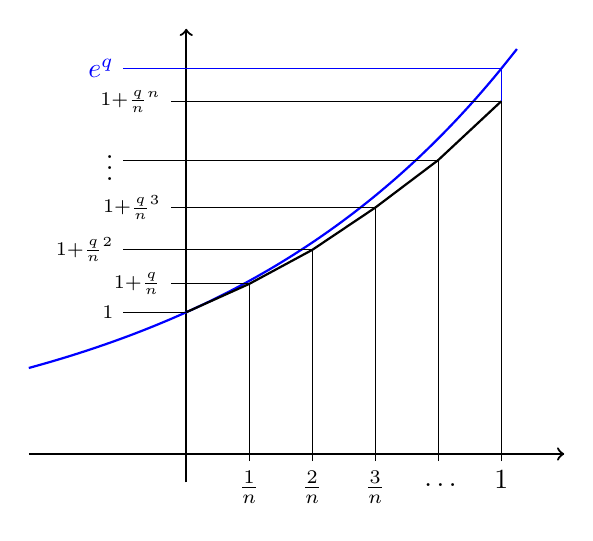
\begin{tikzpicture}[x=4.0cm,y=1.8cm]
    	\draw[thick,->] (-0.5,0) -- (1.2,0);
      \draw[thick,->] (0,-0.2) -- (0,3.0);
      %
      \draw[domain=-0.5:1.05,smooth,variable=\x,thick,blue] plot
      ({\x}, {exp(\x)});
      \draw[blue] (1.0,-0.05) -- (1.0,{exp(1.0)})
      -- (-0.2, {exp(1.0)}) node[left]{$e^q$};
      \draw (-0.2,1) node[left]{$\scriptstyle 1$} -- (0,1);
      \draw (0.2,-0.05) node[below]{$\frac 1 n$} -- (0.2,1.2)
      -- (-0.05,1.2) node[left]{$\scriptstyle 1+\frac q n$};
      \draw (0.4,-0.05) node[below]{$\frac 2 n$} -- (0.4,1.44)
      -- (-0.2,1.44) node[left]{$\scriptstyle\enclose{ 1+\frac q n}^2$};
      \draw (0.6,-0.05) node[below]{$\frac 3 n$} -- (0.6,1.738)
      -- (-0.05,1.738) node[left]{$\scriptstyle\enclose{1+\frac q n}^3$};
      \draw (0.8,-0.05) node[below]{$\rule{0mm}{2mm}\dots$} -- (0.8,2.0736)
      -- (-0.2,2.0736) node[left]{$\vdots$};
      \draw (1.0,-0.05) node [below] {$1$} -- (1.0,2.48832)
      -- (-0.05,2.48832) node[left]{$\scriptstyle\enclose{1+\frac q n}^n$};
      \draw[thick] (0,1) -- (0.2,1.2)
      -- (0.4,1.44) -- (0.6,1.738)
      -- (0.8,2.0736) -- (1.0,2.48832);
    \end{tikzpicture}
  \end{center}
  \caption{Compound interest.
  If we divide the interval $[0,1]$
  into $n$ parts (in the figure $n=5$), at step zero
  we start with a capital equal to $1$, and at each
  step of width $\frac 1 n$, we multiply
  our capital by $1+\frac q n$ (assuming
  we have an interest rate of $q$ that
  in the time $\frac 1 n$ pays us $\frac q n$
  times our capital).
  After
  $n$ steps, i.e., at time $1$, we will have
  a capital equal to $\enclose{1+\frac q n}^n$.
  If $n\to+\infty$, this quantity tends to $e^q$.}
  \label{fig:nepero}
\end{figure}


The exponential function is linked to a growth model often found
in nature: \emph{exponential growth}%
\mymargin{exponential growth}%
\index{growth!exponential}.
Take, for example, a population of bacteria that grows without
limitations of space and nourishment, or
consider the growth of a capital due to a financial return.

Suppose that a population that at time $t_0=0$
amounts to a certain number $c$ of bacteria, at time
$t>0$ reaches a size $q(t,c)$.
If I let the population grow for an additional
time $s>0$, I will find at time $t+s$ the same
population I would have at time $s$ if at time
zero I had started with the population $q(t)$:
\[
  q(t+s,c) = q(s,q(t,c)).
\]
The previous equation is called the property
of a continuous \emph{semigroup}%
\index{semigroup}.
But fixed $t$, the population $q(t,c)$ must
be proportional to $c$ because each bacterium
has its own offspring independently of the total size
of the population. In practice,
we must have $q(t,c) = k(t) \cdot c$ for some
function $k(t)$ that does not depend on $c$.
Thus,
\[
  q(t+s,c)
  = q(s,q(t,c))
  = k(s) \cdot q(t,c)
  = k(s) \cdot k(t) \cdot c
\]
from which
\[
  k(t+s) = k(s) \cdot k(t).
\]
Based on theorem~\ref{th:isomorfismo},
we can assert
that $k(t)$ is an exponential function $k(t)=a^t$
for some constant $a$.
The constant $a$ can be determined using the formula:
\[
  a = k(1) = \frac{q(1,c)}{c}
\]
but this expression does not have a precise physical meaning because
it depends on the unit of time chosen.

The constant to which we can give meaning is instead the instantaneous relative
increase of the population. We can indeed assume that
if we let the population grow for a very small time $\Delta t$,
we will obtain a population increase proportional to the time $\Delta t$
and the population:%
\mynote{%
We are here anticipating the concept of derivative}
\begin{equation}\label{eq:488464}
  q(\Delta t,c) = c + r c \Delta t = (1+r \Delta t) c.
\end{equation}
The constant $r$ thus represents the instantaneous
relative increase of the population (in the case of investment,
$r$ would be the instantaneous interest rate).
This definition makes sense
when $\Delta t$ is small because it does not take into account the fact that
in the time interval $[t,t+\Delta t]$, the population that has
been added also generates new population (i.e., the accumulated interest
also generates interest\mynote{%
In fact, the discovery of the constant $e$
is due to Jacob Bernoulli (1655--1705), see historical notes 
on page~\pageref{note:Bernoulli}}).

To calculate the population increase over "large" times, we can
divide the time intervals into $n$ small intervals of width
$\Delta t$ and apply the relation \eqref{eq:488464} in each of them.
We find:
\begin{align*}
 q(\Delta t,c) &= c(1+r\Delta t) \\
 q(2\Delta t,c) &= q(\Delta t,c) (1+r\Delta t)  = c(1+r\Delta t)^2\\
 &\vdots \\
 q(n\Delta t) &= c(1+r\Delta t)^n.
\end{align*}
Thus, setting $\Delta t=t/n$, we have
\[
  q(t,c) = c\enclose{1+r\frac{t}{n}}^n
\]
in particular for $t=1/r$, we obtain:
\[
  q(1/r,c) = c\enclose{1+\frac{1}{n}}^n
\]
and remembering that $q(t,c)=c a^t$, we obtain:
\[
  a^{\frac 1 r} = \enclose{1+\frac{1}{n}}^n.
\]
If for $n\to +\infty$ (which corresponds to $\Delta t \to 0$)
the quantity on the right tends to a number $e$ (which we will call the Napier's
constant), we will then have
\[
  a = e^r, \qquad q(t,c) = c e^{rt}
\]
which is the relation that links the two constants $a$ and $r$ that define
exponential growth.

The following is indeed valid.

\begin{theorem}[Napier's constant]
\mymark{**}%
\label{th:5767684}
The sequence
\[
  a_n = \enclose{1+\frac 1 n}^n
\]
is increasing and bounded, thus it is convergent.
\end{theorem}
%
To prove the previous theorem, we need 
the following preliminary result.
%
\begin{theorem}[Bernoulli's inequality]
  \label{th:disuguaglianza_bernoulli}%
  \mymark{**}%
  \mymargin{Bernoulli's inequality}%
  \index{Bernoulli!inequality}%
  \index{inequality!Bernoulli's}%
  If $x > -1$ and $n\in \NN$, we have
  \begin{equation}
  \label{eq:bernoulli}
  (1+x)^n \ge 1 + nx.
  \end{equation}
  \end{theorem}
  %
  \begin{proof}
  \mymark{**}
  We prove that~\eqref{eq:bernoulli}
  holds by induction on $n$.
  For $n=0$, the inequality \eqref{eq:bernoulli} becomes $1\ge 1$
  and is therefore verified.
  If~\eqref{eq:bernoulli}
  is verified for a certain $n$,
  multiplying both sides by $1+x > 0$, we obtain
  \[
  (1+x)^{n+1} \ge (1+x) (1+nx) = 1 + (n+1)x + n x^2
  \ge 1 + (n+1)x
  \]
  which is precisely the inequality~\eqref{eq:bernoulli}
  with $n+1$ in place of $n$.
  \end{proof}
%
\begin{proof}[Proof of Theorem~\ref{th:5767684}]
First, we prove that $a_n$ is increasing, i.e., that
for every $n\ge 2$, we have $a_n \ge a_{n-1}$.
It is clear that $a_n>0$ for every $n$,
so we reduce to
verifying that $\frac{a_n}{a_{n-1}} \ge 1$.

We have
\begin{align*}
\frac{a_n}{a_{n-1}}
&= \frac{\enclose{1+\frac 1 n}^n}{\enclose{1+\frac 1 {n-1}}^{n-1}}
= \frac{\enclose{\frac{n+1}{n}}^n}{\enclose{\frac{n}{n-1}}^{n-1}}\\
&= \enclose{\frac{n+1}{n}\cdot\frac{n-1}{n}}^n \cdot \frac{n}{n-1}
= \enclose{\frac{n^2- 1}{n^2}}^n \cdot \frac{n}{n-1}
\end{align*}
Now observe that Bernoulli's inequality, 
Theorem~\ref{th:disuguaglianza_bernoulli},
guarantees
\[
  \enclose{\frac{n^2 -1}{n^2}}^n
  = \enclose{1-\frac{1}{n^2}}^n
  \ge 1 - \frac{n}{n^2} = 1 - \frac{1}{n} = \frac{n-1}{n}
\]
from which we obtain, as we wanted, $a_n / a_{n-1} \ge 1$, i.e.,
$a_n$ is increasing.

If we now consider the sequence
\[
  b_n = \enclose{1+\frac 1 n}^{n+1}
\]
we observe that we have
\[
  b_n = \enclose{1+\frac 1 n}^n \cdot \enclose{1+\frac 1 n}
   = a_n\cdot \enclose{1+\frac 1 n} > a_n.
\]
To prove that $a_n$ is bounded, it will therefore be sufficient to prove
that $b_n$ is upper bounded. We will now see that $b_n$ is decreasing (and
therefore $a_n \le b_n \le b_1$ is upper bounded).

We proceed similarly to what was done for $a_n$:
\begin{align*}
\frac{b_{n-1}}{b_n}
& = \frac{\enclose{1+\frac{1}{n-1}}^n}{\enclose{1+\frac{1}{n}}^{n+1}}
  = \frac{\enclose{\frac{n}{n-1}}^n}{\enclose{\frac{n+1}{n}}^{n+1}}
  = \enclose{\frac{n}{n-1}\cdot\frac{n}{n+1}}^{n+1}\cdot\frac{n-1}{n} \\
& = \enclose{\frac{n^2}{n^2-1}}^{n+1} \cdot \frac{n-1}{n}
  = \enclose{1 + \frac{1}{n^2-1}}^{n+1} \cdot \frac{n-1}{n}.
\end{align*}
According to Bernoulli's inequality, we obtain
\[
  \enclose{1 + \frac{1}{n^2-1}}^{n+1}
  \ge 1 + (n+1) \cdot \frac{1}{n^2-1}
  = 1 + \frac{1}{n-1} = \frac{n}{n-1}.
\]
Putting together the two estimates, we thus obtain $b_{n-1}/b_n \ge 1$,
which is what we needed to prove.
\end{proof}

The following is thus justified.

\begin{definition}[Napier's constant]
\mymark{***}
We define the \emph{Napier's constant}%
\mymargin{Napier's constant}%
\index{constant!Napier's}%
\index{$e$}%
\mynote{John Napier (1550-1617), see historical notes on page~\pageref{nota:Nepero}}%
\[
  e = \lim_{n\to +\infty} \enclose{1+\frac 1 n}^n,
  \qquad n\in\NN.
\]
\end{definition}

Knowing that
\[
  \enclose{1+\frac 1 n}^n \le e \le \enclose{1+\frac 1 n}^{n+1}
\]
and setting $n=1$, we obtain $2\le e \le 4$.

\begin{exercise}\label{ex:4876765}
Let $a_n = \frac{n^n}{n!}$ show that $\frac{a_{n+1}}{a_n} \to e$.
\end{exercise}


\begin{theorem}[limits reducible to the number $e$]
\mymargin{limits reducible to the number $e$}%
\index{limits reducible to the number $e$}
We have 
\[
\lim_{x\to 0}  \enclose{1 + x}^{\frac 1 {x}} = e.
\]
\end{theorem}
%
\begin{proof}
  We start by proving that 
  \begin{equation}\label{eq:2373793}
    \lim_{x\to +\infty} \enclose{1+\frac 1 x}^x = e.
  \end{equation}
  Every real number $x$ is between two consecutive integers:
  \[
      \lfloor x \rfloor \le x \le \lfloor x\rfloor + 1
  \]
  and thus
  \[
    1+\frac{1}{\lfloor x\rfloor +1 } 
    \le 1 + \frac 1 x 
    \le 1 + \frac 1 {\lfloor x\rfloor} 
  \]
  from which 
  \begin{equation}\label{eq:48675248}
    \enclose{1+\frac{1}{\lfloor x\rfloor +1 }}^{\lfloor x\rfloor} 
    \le \enclose{1 + \frac 1 x }^x
    \le \enclose{1 + \frac 1 {\lfloor x\rfloor}}^{\lfloor x\rfloor +1}. 
  \end{equation}
  To calculate the limit of the expression on the left, 
  we perform the change of variable $n=\lfloor x\rfloor + 1$ to 
  obtain:
  \begin{align*}
  \lim_{x\to+\infty} \enclose{1+\frac{1}{\lfloor x\rfloor +1 }}^{\lfloor x\rfloor}
  &= \lim_{n\to +\infty} \enclose{1+\frac 1 n}^{n-1}\\
  &= \lim_{n\to +\infty} \frac{\enclose{1+\frac 1 n}^{n}}{1+\frac 1 n}
   = \frac{e}{1} = e.
  \end{align*}
  Similarly, for the limit of the expression on the right, 
  we can perform the change of variable $n=\lfloor x\rfloor$:
  \begin{align*}
    \enclose{1 + \frac 1 {\lfloor x\rfloor}}^{\lfloor x\rfloor +1}
    &= \lim_{n\to+\infty} \enclose{1+\frac 1 n}^{n+1} \\
    &= \lim_{n\to+\infty} \enclose{1+\frac 1 n}^n 
    \cdot \enclose{1 + \frac 1 n} 
    = e \cdot 1 = e.
  \end{align*}
  Thus, by the squeeze theorem, we obtain
  that the expression 
  in the middle of~\eqref{eq:48675248} also tends to $e$.
  As a consequence, through the change of variable $x\mapsto \frac 1 x$,
  we obtain 
  \[
  \lim_{x\to 0^+}\enclose{1+x}^{\frac 1 x} = e.  
  \]

  Now consider the limit as $x\to -\infty$ 
  of the usual expression. 
  Through the change of variable $y=-x$, we have 
  \begin{align*}
  \lim_{x\to -\infty} \enclose{1+\frac{1}{x}}^x 
  &= \lim_{y\to +\infty} \enclose{1 - \frac 1 y}^{-y}
   = \lim_{y\to +\infty} \enclose{\frac {y-1} y}^{-y}\\
  &= \lim_{y\to +\infty} \enclose{\frac{y}{y-1}}^y
   = \lim_{y\to +\infty} \enclose{1 + \frac{1}{y-1}}^y\\
  &= \lim_{y\to +\infty} \enclose{1 + \frac{1}{y-1}}^{y-1}
    \cdot\enclose{1+\frac 1 {y-1}} 
    = e\cdot 1 = e.\\
  \end{align*}
  Consequently, by making the change of variable $x\mapsto \frac 1 x$, 
  we obtain
  \[
  \lim_{x\to 0^-} \enclose{1+x}^{\frac 1 x} = e.
  \]
    Combining the right and left limits, we finally obtain the complete limit as
  $x\to 0$.
\end{proof}
%
\begin{corollary}%
\label{cor:limite_notevole_ex}%
\mymark{**}%
For every $x\in \RR$, we have
\[
  \lim_{n\to +\infty} \enclose{1+ \frac x n}^n = e^x.
\]
\end{corollary}
%
\begin{proof}
Indeed, by the previous theorem, setting $y = x/n$, we have
$y\to 0$ as $n\to +\infty$, and therefore
\[
\lim_{n\to +\infty}\enclose{1+\frac x n}^{\frac n x} 
= \lim_{y\to 0} \enclose{1+y}^{\frac 1 y}
= e.
\]
But then
\[
\enclose{1+ \frac x n}^n = \enclose{\enclose{1+\frac x n}^{\frac n x}}^x
\to e^x
\]
\end{proof}

\begin{definition}[natural logarithms]
We will see that the number $e$ turns out to be a natural base for the
exponential
function and consequently for the logarithm. The logarithm to base
$e$ is called the \emph{natural logarithm}%
\mymargin{natural logarithm}%
\index{logarithm!natural} and is denoted by $\ln = \log_e$.
\end{definition}

\mynote{%
In some texts, the operator $\log$ is used, indicated without an explicit base,
but the definition is not completely shared.
In certain texts (mostly in the mathematical field),
$\log  = \ln = \log_e$ is defined,
while in other texts, $\log = \log_{10}$ is considered.
}

\begin{corollary}[notable limits]\label{cor:limite_notevole_e}
\mymark{*}%
We have
\begin{gather}
 \lim_{x\to 0} \frac{\ln \enclose{1+ x}}{x} = 1; \\
 \lim_{x\to 0} \frac{e^x-1}{x} = 1.
\end{gather}
\end{corollary}
%
\begin{proof}
Regarding the logarithm, we reduce to the previous theorem
by observing that:
\[
  \frac{\ln(1+x)}{x}
  = \ln \enclose{(1+x)^{\frac 1 {x}}}
  \to \ln e = 1.
\]
For the exponential, we reduce to the logarithm
by observing that setting
\[
  y = e^x-1
\]
if $x\to 0$, then $y\to 0$, and therefore we have:
\[
\frac{e^{x}-1}{x} = \frac{y}{\ln(1+y)} \to 1.
\]

\end{proof}

\begin{exercise}
Show that
\begin{gather*}
  \lim_{n\to+\infty} n^n\cdot \enclose{\frac{n+1}{n^2+1}}^n = e; \\
  \lim_{n\to+\infty} n\cdot \ln\enclose{1 + \frac 1 n} = 1; \\
  \lim_{n\to+\infty} \enclose{1-\frac{n+1}{n!}}^{(n-1)!} = \frac 1 e; \\
  \lim_{n\to+\infty} n \cdot \enclose{\sqrt[n]{2}-1} = \ln 2.
\end{gather*}
\end{exercise}

%%%%%%%%%%%%%%%%%%%
%%%%%%%%%%%%%%%%%%%
%%%%%%%%%%%%%%%%%%%
%%%%%%%%%%%%%%%%%%%
\subsection{Ratio and Root Tests}

It often happens that we need to determine the limit
of the ratio of two sequences that both tend to infinity
or both tend to zero.
In these situations, the theorem of the limit of the ratio does not
apply because we are faced with an indeterminate form.
We must therefore understand which of the two sequences
tends to infinity or zero "more quickly."

The following theorems are based (more or less implicitly)
on the behavior of the geometric sequence:
\[
  a_n = q^n
\]
where $q>0$ is a fixed constant.
From the properties of the exponential function, 
we know that if $q>1$, we have $q^n\to \infty$.
If $q=1$, clearly $q^n=1\to 1$,
and if $q<1$, we have $q^{-1}>1$, and therefore $q^{-n} \to +\infty$,
from which $q^n \to 0$.

\begin{theorem}[ratio test]
\label{th:criterio_rapporto}
\index{test!ratio for sequences}
\index{ratio!test of}
  Let $a_n$ be a real sequence with positive terms
  $a_n > 0$ such that the limit of the ratio of two consecutive terms exists:
  \[
     \frac{a_{n+1}}{a_n} \to \ell \in [0,+\infty].
  \]
  If $\ell < 1$, then $a_n \to 0$; if $\ell >1$, then $a_n \to +\infty$.
\end{theorem}
%
%
% \begin{proof}\mynote{%
%   the proof of this theorem could be done in a manner
%   very similar to the proof of theorem~\ref{th:criterio_radice}
%   without invoking theorem~\ref{th:criterio_cesaro}, which is decidedly more complex.
%   }
% Thanks to theorem~\ref{th:criterio_cesaro}, we know
% that $\sqrt[n]{a_n}\to \ell$, and therefore the result
% follows directly from theorem~\ref{th:criterio_radice}.
% \end{proof}
%

\begin{proof}
Suppose $\ell<1$. Set $q=(1+\ell)/2$, so $\ell < q < 1$, 
and set $\eps=q-\ell>0$. By the definition of limit $\frac{a_{n+1}}{a_n}\to
\ell$,
there must exist an $N\in \NN$ such
that for every $n\ge N$, we have:
\[
  \frac{a_{n+1}}{a_n} < \ell + \eps = q
\]
i.e., $a_{n+1} < q \cdot a_n$. In particular, we will have:
\begin{align*}
  a_{N+1} &< q \cdot a_N \\
  a_{N+2} &< q \cdot a_{N+1} < q^2\cdot a_N \\
  a_{N+3} &< q \cdot a_{N+2} < q^3\cdot a_N \\
  \vdots
\end{align*}
and it is clear that by induction, we can prove that for
every $k\in \NN$, we have
\[
  a_{N+k} < q^k\cdot a_N.
\]
However, observe that $q^k \cdot a_N \to 0$ as $k\to +\infty$
since $q<1$, and therefore $q^k \to 0$. 
Thus, except for the first $N$ terms, the sequence $a_n$ tends to zero. 
But the first $N$ terms do not affect either the character or the limit 
of the sequence, and therefore the entire sequence $a_n$ tends to zero.

The case $\ell>1$ is handled similarly. Choose $q$ such
that $1<q<\ell$, and find, similarly to the previous case,
that for a certain $N\in \NN$ and for every $k\in \NN$, we have
\[
  a_{N+k} > q^k \cdot a_N \to +\infty.
\]
\end{proof}

Note that, in the previous theorem (but also in the root test
theorem~\ref{th:criterio_radice}),
nothing can be concluded in
the case where $\ell = 1$.
For example, the two sequences $a_n = 1/n$ and $b_n = n$
have different limits ($a_n \to 0$, $b_n\to +\infty$), but for both,
the limit of the ratio of consecutive terms tends to $\ell=1$.

\begin{exercise}
Show that
\begin{gather*}
  \lim \frac{n!}{n^n} = 0 \\
  \lim \frac{(2n)!}{(2n)^n} = +\infty
\end{gather*}
\end{exercise}

\begin{theorem}[root test]
\label{th:criterio_radice}%
\mymark{***}%
\mymargin{root test}%
\index{test!root for sequences}%
Let $a_n$ be a sequence with non-negative terms, $a_n\ge 0$, such that
\[
  \sqrt[n]{a_n} \to \ell
\]
with $\ell \in \bar \RR$.
Then if $\ell<1$, we have $a_n \to 0$; if $\ell > 1$, we have $a_n \to +\infty$.
\end{theorem}
%
\begin{comment}
\begin{proof}
\mymark{**}
Consider first the case $\ell < 1$.
If $\lim \sqrt[n]{a_n} = \ell$, it means that for every $\eps>0$, the sequence
$\sqrt[n]{a_n}$ is definitively less than $\ell +\eps$.
Choosing $\eps$ appropriately (e.g., $\eps = (1-\ell)/2$), we can
have $q = \ell+\eps < 1$. Thus, we will have definitively $\sqrt[n]{a_n}< q$,
i.e., $a_n < q^n$. By hypothesis, $a_n\ge 0$,
and therefore, except for a finite number of terms, we have $0 \le a_n < q^n \to
0$,
from which $a_n \to 0$ (since removing a finite number of terms does not
change either the character or the limit of the sequence).

If $\ell>1$, we can proceed similarly. There will exist $q$ with $1 < q < \ell$
such that definitively $\sqrt[n]{a_n} > q$, from which $a_n > q^n \to +\infty$.
\end{proof}
\end{comment}

\begin{proof}
  It can be observed that
  \[
    a_n = \enclose{\sqrt[n]{a_n}}^n
     = e^{n \cdot \ln \sqrt[n]{a_n}}.
  \]
  If $\ell <1$, then the logarithm tends to a negative number,
    the argument of the exponential tends to $-\infty$, and therefore the
  exponential tends to zero.

    If instead $\ell>1$, the logarithm tends to a positive number, and therefore
  the exponential tends to $+\infty$.
\end{proof}

%%%%%
%%%%%